\begin{frame}[label=Lebesgue]
  \frametitle{Lebesgue}
  \begin{block}{Nuovi problemi}    
    La scoperta di Riemann dell'esistenza di funzioni integrabili con un insieme denso di punti di discontinuità
    pose la seguente questione: \say{esiste un concetto più generale di integrale?}. L'espressione 
      $\int^1_0 \mathcal{D} (x) dx $
    ha un significato?
  \end{block}  
  \begin{block}{Generalizzazione del concetto di integrale}
    Lebesgue (1902) propose che l'area sottesa ad una curva poteva essere approssimata con un insieme \textit{infinito} (in atto)
    di rettangoli, e questo fa una grande differenza. 
    \begin{wrapfigure}{r}{0.3\textwidth}
    \begin{center}
      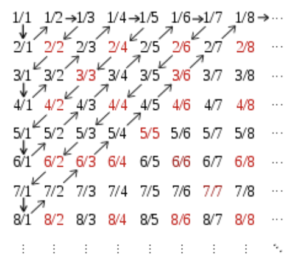
\includegraphics[scale=.3]{numQ.png}
    \end{center}
    \end{wrapfigure}        Data la funzione 
    \begin{equation*}
      \mathcal{D}(x) =
      \begin{cases*}
        1 & se x è razionale \\
        0 & se x è irrazionale
      \end{cases*}
    \end{equation*}

    l'area sottesa al grafico $y=\mathcal{D} (x)$ nell'intervallo $[0,1]$ è l'area che sta sotto i punti per qui $\mathcal{D} (x)=1$; 
    gli altri non danno contributo all'area. Tali punti sono i razionali del'intervallo $[0,1]$ che sono un insieme \textit{numerabile}.
    \begin{center}
      $\frac{1}{2},\frac{1}{3},\frac{2}{3},\frac{1}{4},\frac{3}{4},...$
    \end{center}
    Prima le frazioni che hanno al denominatore 2, poi quelle che hanno al denominatore 3, poi 4, 5 e così via.
  \end{block}  
\end{frame}      


\begin{frame}
  \frametitle{Lebesgue}
    \begin{block}{Generalizzazione del concetto di integrale (...segue)}
    Al punto $x$, razionale, corrisponde una linea verticale. Se pensiamo di racchiudere questa linea con un rettangolo di altezza $1=\mathcal{D} (x)$ 
    e per base $\frac{\epsilon}{2^n}$ per $n \in \mathbb{N} $. L'area è quindi ricoperta di rettangoli la cui somma è
    \begin{center}
      $\frac{\epsilon}{2}+\frac{\epsilon}{4}+\frac{\epsilon}{8}+\frac{\epsilon}{16}+\frac{\epsilon}{32}+... = \epsilon$
    \end{center}     
    Poiché possiamo segliere $\epsilon$ piccolo a piacere, il valore di quest'area tende a 0. Quindi 
    \begin{center}
      $\int^1_0 \mathcal{D} (x) dx = 0$
    \end{center} 
    quando l'integrale è inteso nel senso di Lebesgue. \\
    Poiché la lunghezza dell'intervallo $[0,1]$ è pari a 1 e l'insieme dei razionali 
    può essere ricoperto da intervalli di lunghezza totale (o \say{misura}) $\epsilon$, 
    l'insieme degli irrazionali ha misura pari a 1. Per questo si dice che che \textit{quasi} tutti i punti di $[0,1]$
    sono irrazionali. \textit{La funzione di Dirichlet $\mathcal{D} (x)$ ha integrale uguale a zero perchè  $\mathcal{D} (x)$ 
    è zero quasi ovunque.}  
  \end{block}
\end{frame}


